% This is the main report file

\documentclass{acm_proc_article-sp}
\usepackage[utf8]{inputenc}
\usepackage{listings}
\usepackage{hyperref}
\usepackage{fancyhdr}

\lhead{
\includegraphics[scale=1.0]{img/header.eps}} \lfoot{
\includegraphics[scale=0.5]{img/footer.eps}}
\begin{document}
\thispagestyle{fancy}% sets the current page style to 'fancy' -- must 
\title{Android based audience response system}
\subtitle{[Technical documentation - version 1.1]
\titlenote{Authors list is available in appendix \ref{app:authors}}
}

\numberofauthors{1}
\author{
\alignauthor DOSSEE team at the Technical university of Denmark
}


\maketitle

\begin{abstract}
The purpose of this document is provide the needed information in order to implement a working prototype within two working weeks.
%Abstract; A brief summary of all of the report including the conclusion section
%but excluding the acknowledgements, references and any appendixes.
\end{abstract}
\section{Introduction}
\label{sec:introduction}
An \textit{Audience Response System} (ARS) allows several participants to cast votes on a particular subject or question from a set of predefined possible answers. More specifically, the ARS allows participants to answer \textit{polls}, which are (unique) voting instances, each having its own set of questions and answer possibilities. The time interval for which answers are accepted to a poll is known a the \textit{voting round}, each giving a unique result to the poll. Note that each poll may have several voting rounds, allowing for the poll to be repeated, possibly producing different results for each voting round. When a voting round has ended, the system collects the answers from the participants and makes a summary of the results available. 

The broad definition of audience response systems allows for many different possible implementations and with vastly different feature sets.

In “Who Wants to be a Millionaire”, such a system is employed when the audience is asked to answer a question to help the participant. Here, the answer possibilities is shown on an interactive touch-screen monitor and all participants are required to answer within a certain time frame.

Applications of such a system can also easily be found in a study scenario. Studies have shown that you get the best result when teaching if you are able to interact with the students. You can do this by asking the students a question during class and then introduce possible answers. The students would have to answer by marking with their hands.  Unfortunately not all students participate in this kind of interacting because they cannot be anonymous, and it can be very difficult to get an overview over many students participated. To solve this problem some universities require the students to buy a clicker device. It is a small remote control looking device that costs about 40\$ and which allows for interaction with an ARS. 

Every clicker device has a wireless connection to the receiver device, connected to the teacher’s laptop. The students are then able to anonymously answer the questions the teacher has prepared. The teacher is then able to generate result statistics and graphs based on how the students answered. This seems like a very good solution. The problem is that every student has to buy such a device and remember it every time they go to class. The Danish project recognises that ARS’s are a valuable resource in many situations, and extends it with a simple idea:

\begin{quote}
\textit{Why not just use a device that they always have in their pocket - a smartphone?}
\end{quote}


%
%Introduction; A discussion putting the work into context and discussing the
%background of the work. The section should include any problem statements
%addressed, a very brief summary of the work carried out, the most import ant
%results and the most important conclusions. The section should end with a
%description of the report structure.



\section{Use cases}
\thispagestyle{fancy}% sets the current page style to 'fancy' -- must 

%TODO multipicities - ex. class diagram
For our usage, two actors has been identified; a student and an teacher.
\begin{figure}[h]
\centering
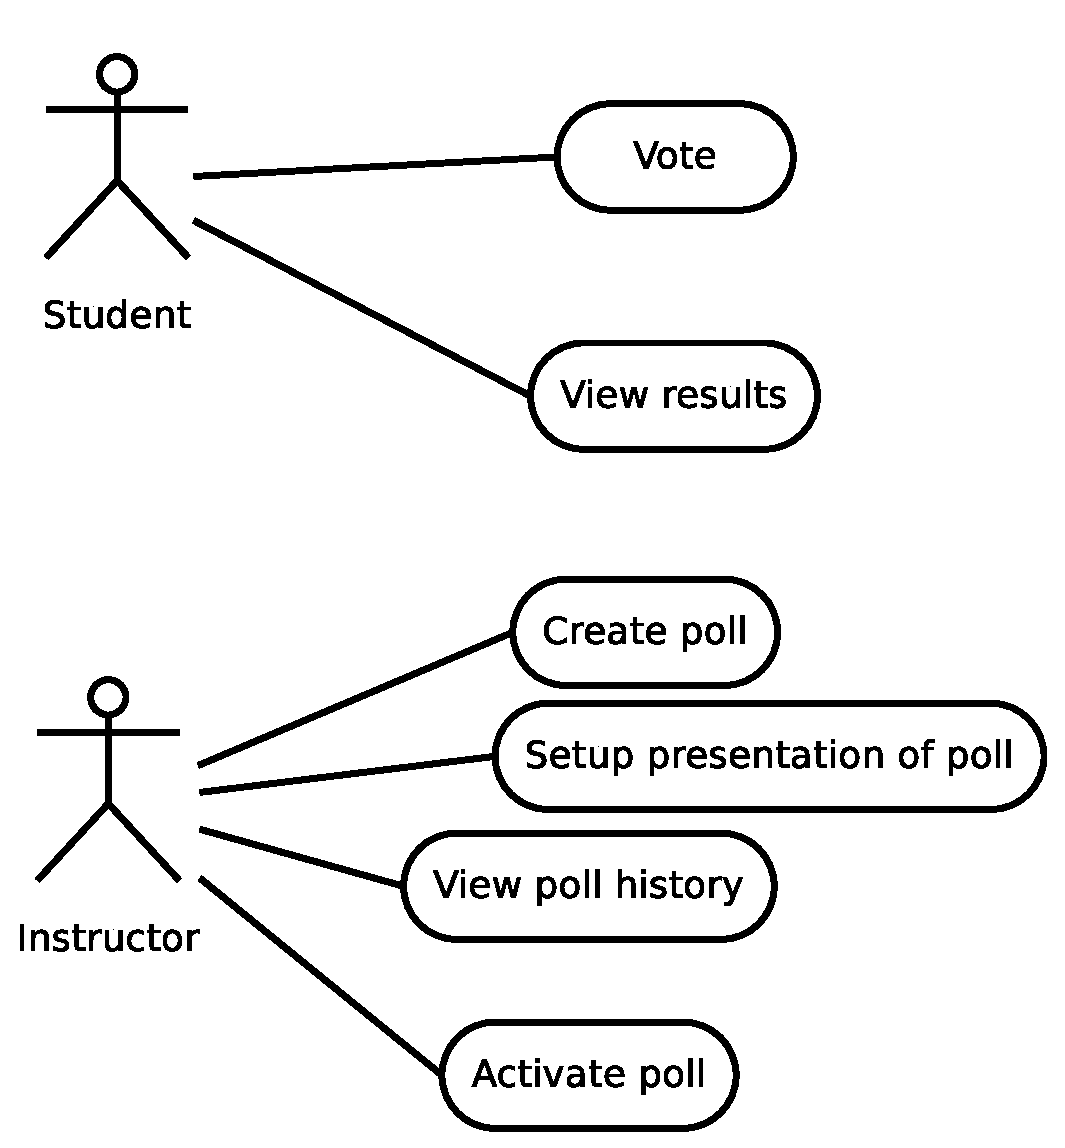
\epsfig{file=fig/use_cases.eps, height=2.0in}
\caption{Use cases}
\label{fig:use_cases}
\end{figure}
The student has access to the intended usage of the system and is considered the normal end-user. The teacher has the administrator role in the sense that he/she is responsible for the back-office operations. For further reference, see figure \ref{fig:use_cases};\\\\

\section{Requirements}
For the system, the following requirements has been identified to support the basic usage of the system
\begin{itemize}
  \item Simple to use
  \item No user login
  \item Multiple choice polls
  \item Persistent storage of polls and results
  \item No live view
  \item Basic semantics
\end{itemize}
An elaboration of each requirement follows
\subsubsection*{Simple to use}
The system must have as little interaction with users as possible. Make as many decisions on predefined values as possible and avoid asking the user.

The system has no notion of persistent users, but instead uses a shared secret scheme in the form of a generated url. This functionality is roughly corresponding the one used at doodle.com.

\subsubsection*{Multiple choice polls}
The system is a basic multiple-choice poll. One question, several answers. Once a poll has been answered by a user, it cannot be replied to again in the same session.
%TODO Check op on this and what the conclusion on the multiple users discussion was.

\subsubsection*{Persistent storage}
The polls and the results must be stored until explicitly removed by the teacher.

\subsubsection*{No live view}
There is no live view option for showing the results before the poll closes. This is due to the fact early poll estimates can have effect on the result.

\subsubsection*{Basic semantics}
The application should a have a notion of right and wrong answers - if applicable.

\subsection{Possible improvements}
This section describes the ideas for improving the general usefulness and quality of the application.
\begin{itemize}
  \item Statistics
  \item Security and authentication
  \item Remote access 
  \item Shared voting devices 
  \item Real questions
  \item Optional user login
\end{itemize}

\subsubsection*{Statistics}
Basically any additional information that goes beyond basic usage. Comparison of results from different polls or poll sessions. This one requires the login functionality to be implemented.

\subsubsection*{Security and authentication}
More security can be added without adding extra complexity.
\subsubsection*{Remote access}
Think webcasts - no physical presense should be required
\subsubsection*{Shared devices}
More than one user has access to polls on single device
\subsubsection*{Real questions}
Use a string for answer for inputting string values other than predefined values.

\subsubsection*{Optional user login}
There could be a real login for users (teachers) letting them have an actual account to keep track of their polls.

\section{Infrastructure}
\thispagestyle{fancy}% sets the current page style to 'fancy' -- must 

\begin{figure}[h]
\centering
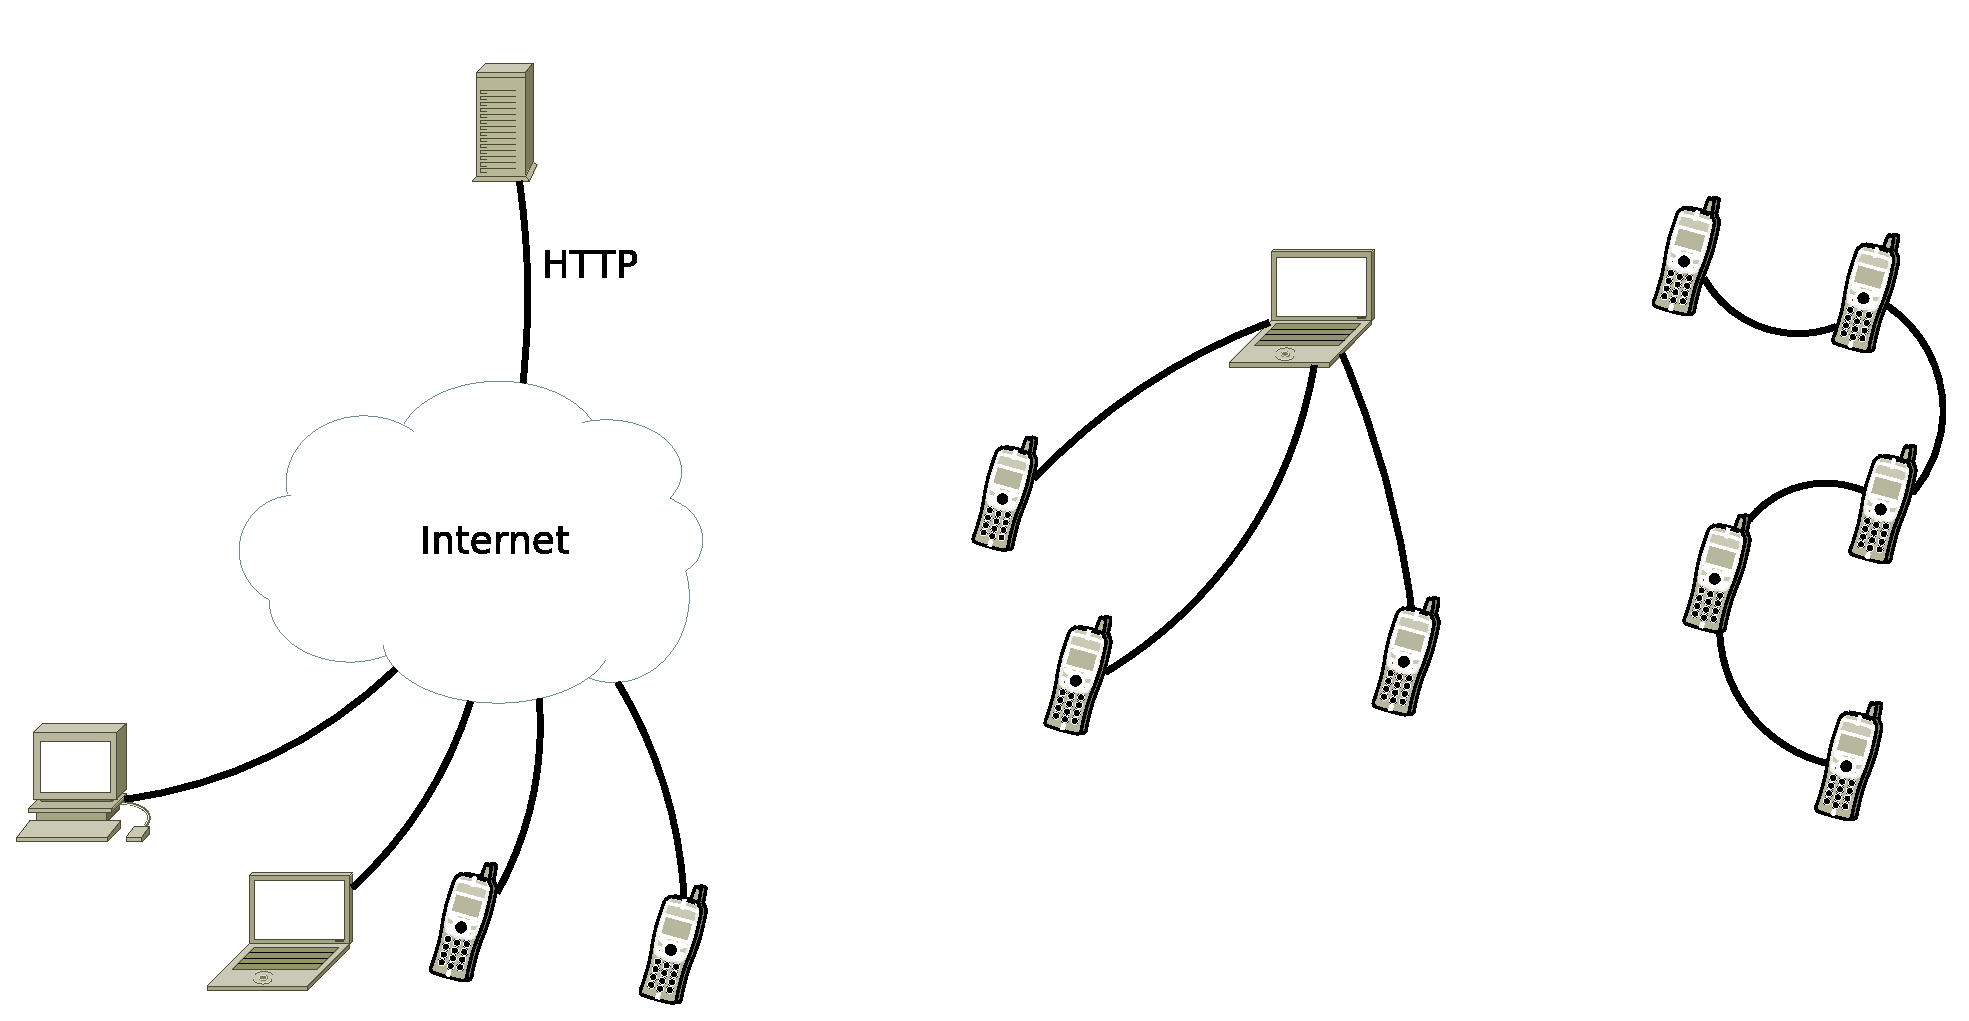
\epsfig{file=fig/architeture_choices.eps, height=1.4in}
\caption{Architeture Choices}
\label{fig:architeture_choices}
\end{figure}

For the network architecture we have chosen a classic client server setup. See diagram for options.

The mesh network was ruled out due to complications with the android ad-hoc networking not being available for non-power users.

The Ad-hoc network was rejected due to the fact that we cannot guarantee the availablilty of the service on various networks and laptops. This is caused by infrastructure security issues - e.g. local firewalls blocking zeroconf/broadcasting.

For using a laptop as access point, it is required that the application has access to the drivers of the laptop in order to change the wireless network card into managed mode. 
On a further note, we are unsure that a laptop is able to handle the number of clients required.




\section{Overall design}

\subsection{Graphical User Interface}
The GUI is in three parts:
\begin{itemize}
  \item Web interface for poll administrators / teachers
  \item (Mobile) web interface for participants / students
  \item Android interface for participants / students
\end{itemize}

A poll, consisting of one or more questions and their answers, is associated with a poll ID and a domain name (for the web interface only).

\subsubsection{Web interface for teachers}
\thispagestyle{fancy}% sets the current page style to 'fancy' -- must 

Both the teacher and student enter the same front page for the web interface by entering the domain name in their browser.

\begin{figure}[h]
\centering
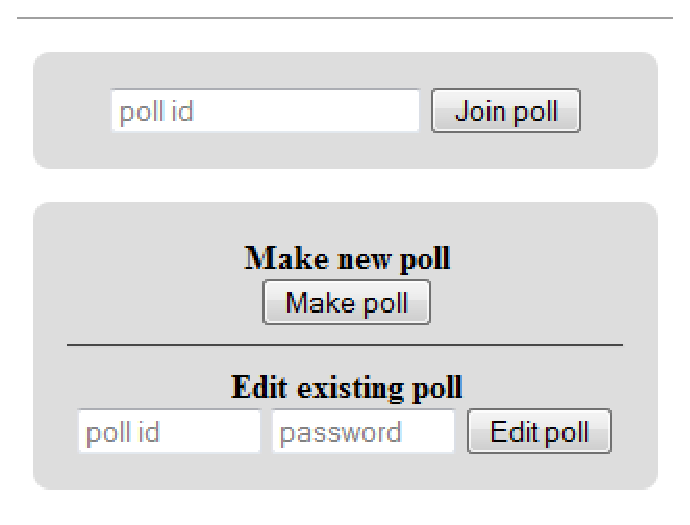
\epsfig{file=fig/teacher_interface.eps, width=200px}
\caption{Log in screen}
\label{fig:teacher_interface}
\end{figure}

A teacher can then create a new poll by clicking Make poll. Poll id and password will then either be chosen by the teacher or mailed to a chosen email address. Making this poll id and password must be quick and easy, like on Doodle.

A teacher can also choose to edit an existing poll if he knows the poll id and password.

\begin{figure}[h]
\centering
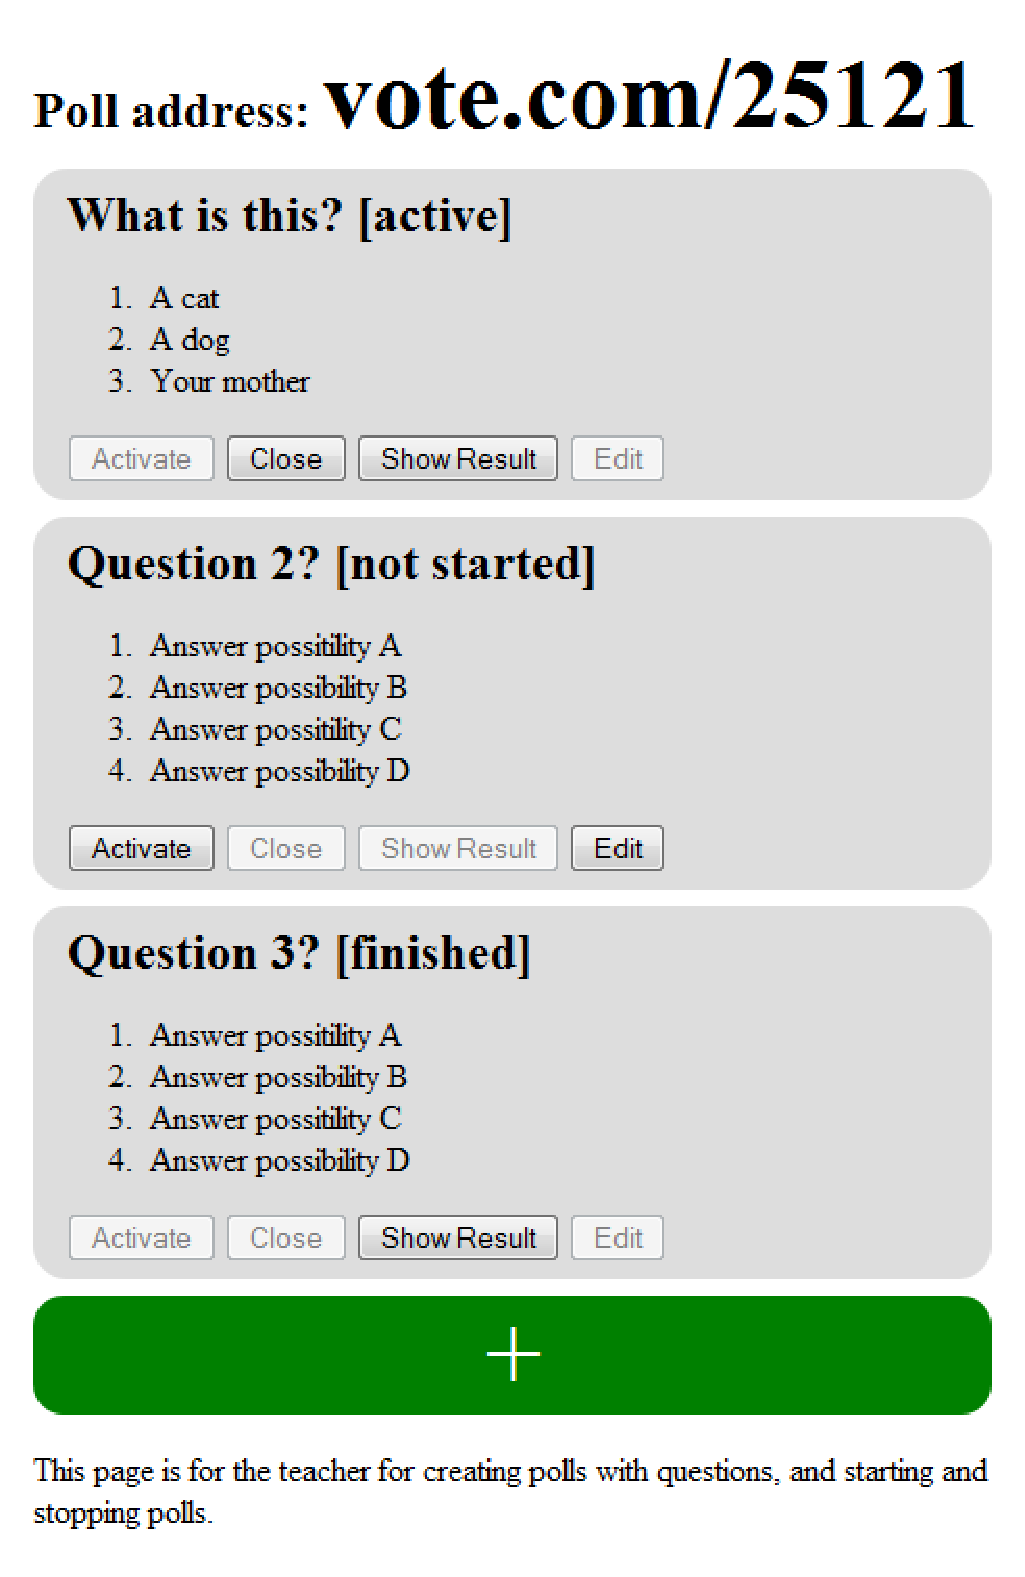
\epsfig{file=fig/polls.eps, width=200px}
\caption{Admin interface}
\label{fig:polls}
\end{figure}

Once the teacher has access to the poll, it is initially empty with only a big green add question (+) button. When adding or editing a question, the teacher can write the question to ask and the number of possible answers, optionally assigning a label to each answer.

The domain and the poll id are shown in the top, which the teacher will hand out to the students by e.g. writing it on the blackboard or in his presentation slides.

\begin{figure}[h]
\centering
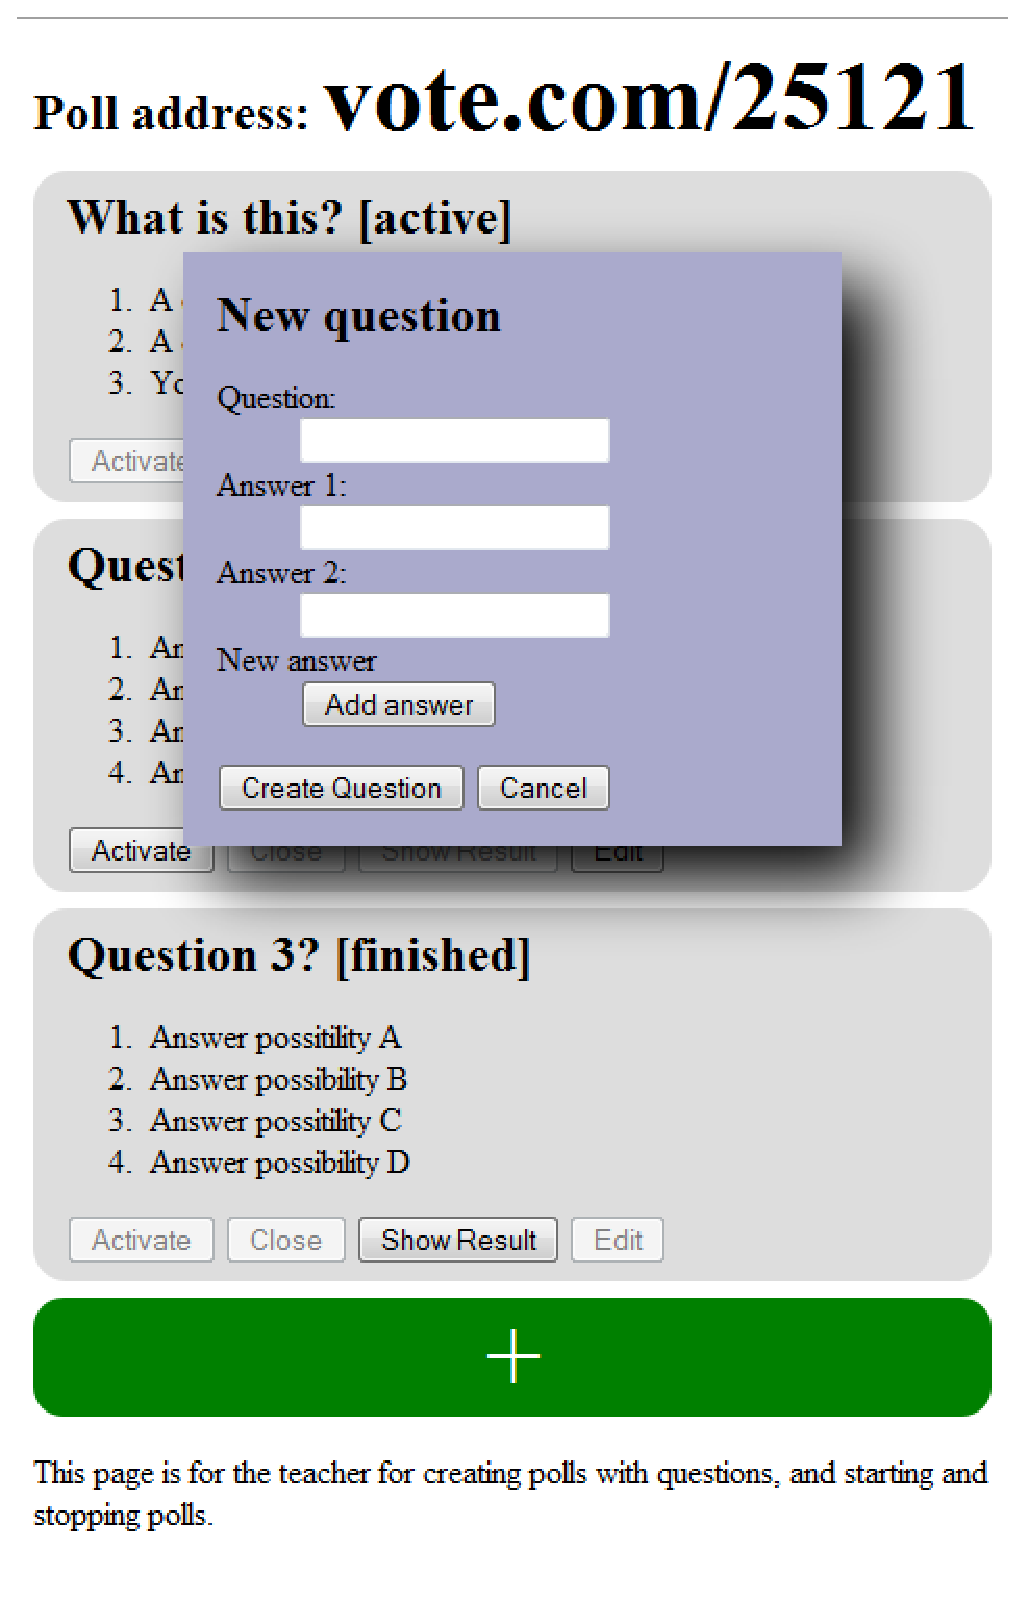
\epsfig{file=fig/new_question.eps, width=200px}
\caption{Creating a new question}
\label{fig:create_question}
\end{figure}
The lifecycle of a question is:
\begin{enumerate}
  \item Action: \textit{The teacher creates a new question.}\\
  The question is now in the not started state where the teacher can edit it and the students cannot see it.
  
  \item Action: \textit{The teacher activates the question.} \\ 
  The question is now in the active state, and will automatically pop up on the screen of each connected student, allowing them to answer.
  \item Action:  \textit{The teacher closes the question.} \\
The question is now in the finished state. It will disappear from the screen of each connected student, and the students will have no more time to answer. The teacher can now view the answers using a number of representations (table, pie chart, …), either on his own screen, on the screen of each student or both.
\end{enumerate}

\subsubsection{Web interface for students}
The student enters the domain name of the voting system into his (mobile or desktop) browser.

\begin{figure}[h]
\centering
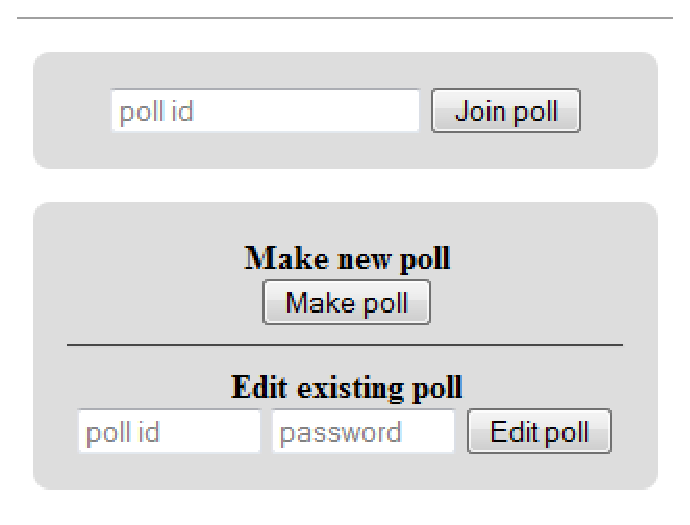
\epsfig{file=fig/teacher_interface.eps, width=200px}
\caption{Log in screen}
\label{fig:teacher_interface}
\end{figure}


The student then sees a screen where he can enter the poll id given by the teacher.

\begin{figure}[h]
\centering
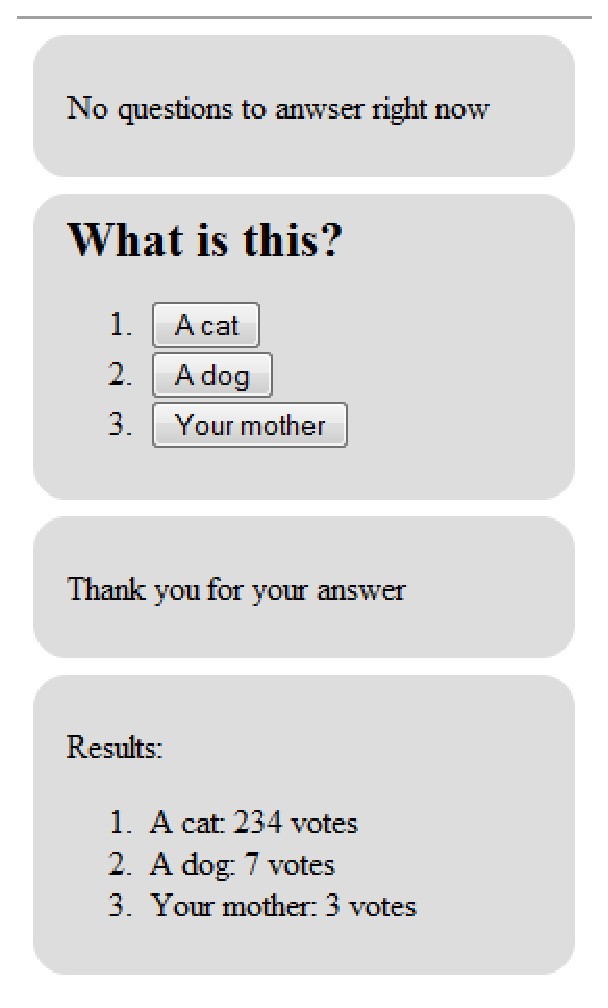
\epsfig{file=fig/poll.eps, width=200px}
\caption{Student view of poll}
\label{fig:poll}
\end{figure}


Initially when the student enters the poll, he just sees a no questions to answer message. Once the teacher decides to ask a question, the question is automatically shown on the screen. When the student answers the question, it disappears with a thank you message. If the student has not yet answered the question when it is closed by the teacher, the question disappears and is replaced with the no questions to answer message. If the teacher decides to show the results of a question, it will automatically show on the screen and stay there until the teacher decides to hide the results.
\subsubsection{Android interface for students}
Unlike the web interface, the student does not have to enter a domain name, as it is already known by the application.

\begin{figure}[h]
\centering

\epsfig{file=fig/android_interface.eps, width=200px}
\caption{Android interface}
\label{fig:android_interface}
\end{figure}

When the student starts up the application, he sees a screen where he can enter the poll id given by the teacher.

Once he has entered the poll id, the rest of the interface is the same as the web interface for students.


\begin{itemize}
  \item A client coded in AJAX that can be accesses via HTTP
  \item A client interface coded in Java for native android phones (an app)
\end{itemize}

\section{Technical Requirements}
\thispagestyle{fancy}% sets the current page style to 'fancy' -- must 

\begin{itemize}
  \item Web server with java
  \item Web server with email sending capabilities
\end{itemize}
Suggested technologies
\begin{itemize}
  \item Template engine (provide a condidate list)
  \item Some framework
  \item JSON/HTTP
  \item AJAX
\end{itemize}
 
\subsection{Template candidates}
\begin{itemize}
 \item Spring MVC
 \item Play
 \item Apache Wicket
 \item Stripes
 \item Grails
 \item Tapestry
\end{itemize}

\subsubsection*{Play - http://www.playframework.org/}

Play is exceptionally easy as no configuration is needed. It uses a stateless model, is ready for REST and is easy scalable. Play uses the groovy scripting language for templating which is build on Java and therefore quick to learn for developers familiar with Java. It provides template inheritance, includes and tags. It integrates easily with Eclipse and other Java IDE's. The Play framework requires Java 5 and Python 2.5 and comes with a built in HTTP server but can also be used with Tomcat and other servers.

\subsubsection*{Spring MVC - http://www.springsource.org/}

Spring MVC relies heavily on XML configuration. There might also be licensing issues with future releases and patches. Due to the heavy configuration needed we suggest only considering this framework if the project leaders have experience with it.

\subsubsection*{Stripes - http://www.stripesframework.org/}

Lightweight and minimal configuration required to get started with a low learning curve. There are however some concerns regarding the available documentation and slow release cycle.

\subsubsection*{Grails - http://www.grails.org/}

Like Play, it is heavily inspired by Ruby on Rails in the development style. The entire frameworks is Groovy based, so it is significantly slower in runtime performance. Using Groovy instead of pure Java does have advantages in terms of development time.

\subsubsection*{Wicket - http://wicket.apache.org/}

Wicket is purely Java based and HTML pages are build only in Java. This might be useful for developers with no knowledge of web developing. But it might seem a bit strict to enforce Java only for everybody in the project group.

\subsubsection*{Tapestry - http://tapestry.apache.org/}

Tapestry reportedly has a very steep learning curve, and both major and minor released often break backwards compatibility forcing an app rewrite.

\subsubsection{Recommendation}

Based on the descriptions above we recommend using the Play framework. We do not have expirience with any of the candidates, but from our point of view Play seems as the most intuitive framework and is easy to get started with. However it might be benificial for the project if the project leaders have expirience with the chosen framework.


\subsection{JSON}
\thispagestyle{fancy}% sets the current page style to 'fancy' -- must 

JSON stands for JavaScript Object Notation, and can be compared to a mix between XML and serialization, understood as JSON being a de-facto standard in many modern webservices, but at the same time, it's a direct way to serialize and deserialize objects without loosing the state. JSON has the advantages of being more lightweight than XML, as well as the possibilities of serializing, sending and then deserializing java objects using the JSON format, rather than having to parse XML. An example of a JSON string could be:

\begin{verbatim}
{"value":42,"hello":"world"}
\end{verbatim}

Which would correspond the JSON representation of an object that has an int field called \texttt{value} with the value 42, and a String field with named \texttt{hello} with the value \texttt{world}:

\begin{verbatim}
class Object {
	protected int value = 42;
	protected String hello = "world";
}
\end{verbatim}

To allow the decoding and encoding of objects, we will use Google's own JSON library; \href{http://code.google.com/p/google-gson/}{gson}. This makes it super simple to work with JSON, since it's possible to just call the following code to serialize and deserialize an object:

\begin{verbatim}
Object obj1 = new Object();

Gson gson = new Gson();
String json = gson.toJson(obj1);
System.out.println(json); 
// {"value":42,"hello":"world"}

Object obj2 = gson.fromJson(json);
// obj2 now has the same instance variables as 
// obj1 had when it was turned into json.
\end{verbatim}

Just like with normal java-serialization, it is possible to exclude fields from the JSON string simply by making them transient, so the following object would still get turned into the JSON string shown above:

\begin{verbatim}
class Object2 {
	protected int value = 42;
	protected String hello = "world";
	protected transient boolean isTheWorldFlat = false;
	protected transient String hot = "dog";
}
\end{verbatim}

Note that it becomes slightly more complicated when dealing with collections or generic types, but it is not that difficult, and since this is a high-activity Google code project, the internet is full of discussions about the different aspects. When using gson, the only required thing is to download and import the classes, and then it's basically plug-and-play.

\balancecolumns
% That's all folks!
 
\section{MessageFlow and Protecol Messages} 
\thispagestyle{fancy}% sets the current page style to 'fancy' -- must 

This section describes the messageflow in the system as well as a description of the messages.
It is adviceable to look at \ref{fig:Messageflow} and \ref{fig:ProtocolMessages} while reading as it will ease understanding.
The client of the system, it being a phone or laptop, it referred to as a "responder". The user using the responder is called a student
The server is referred to as a pollprovider and the person controlling it is a "teacher".

Note: when looking at the diagrams, be aware that there is a difference between \subsection{QuestionAnswer} and \subsection{QuestionResult}
The first is the answer the students sends to a question, and the second the factual results given by the teacher to the student. 

\begin{figure}[h]
\centering
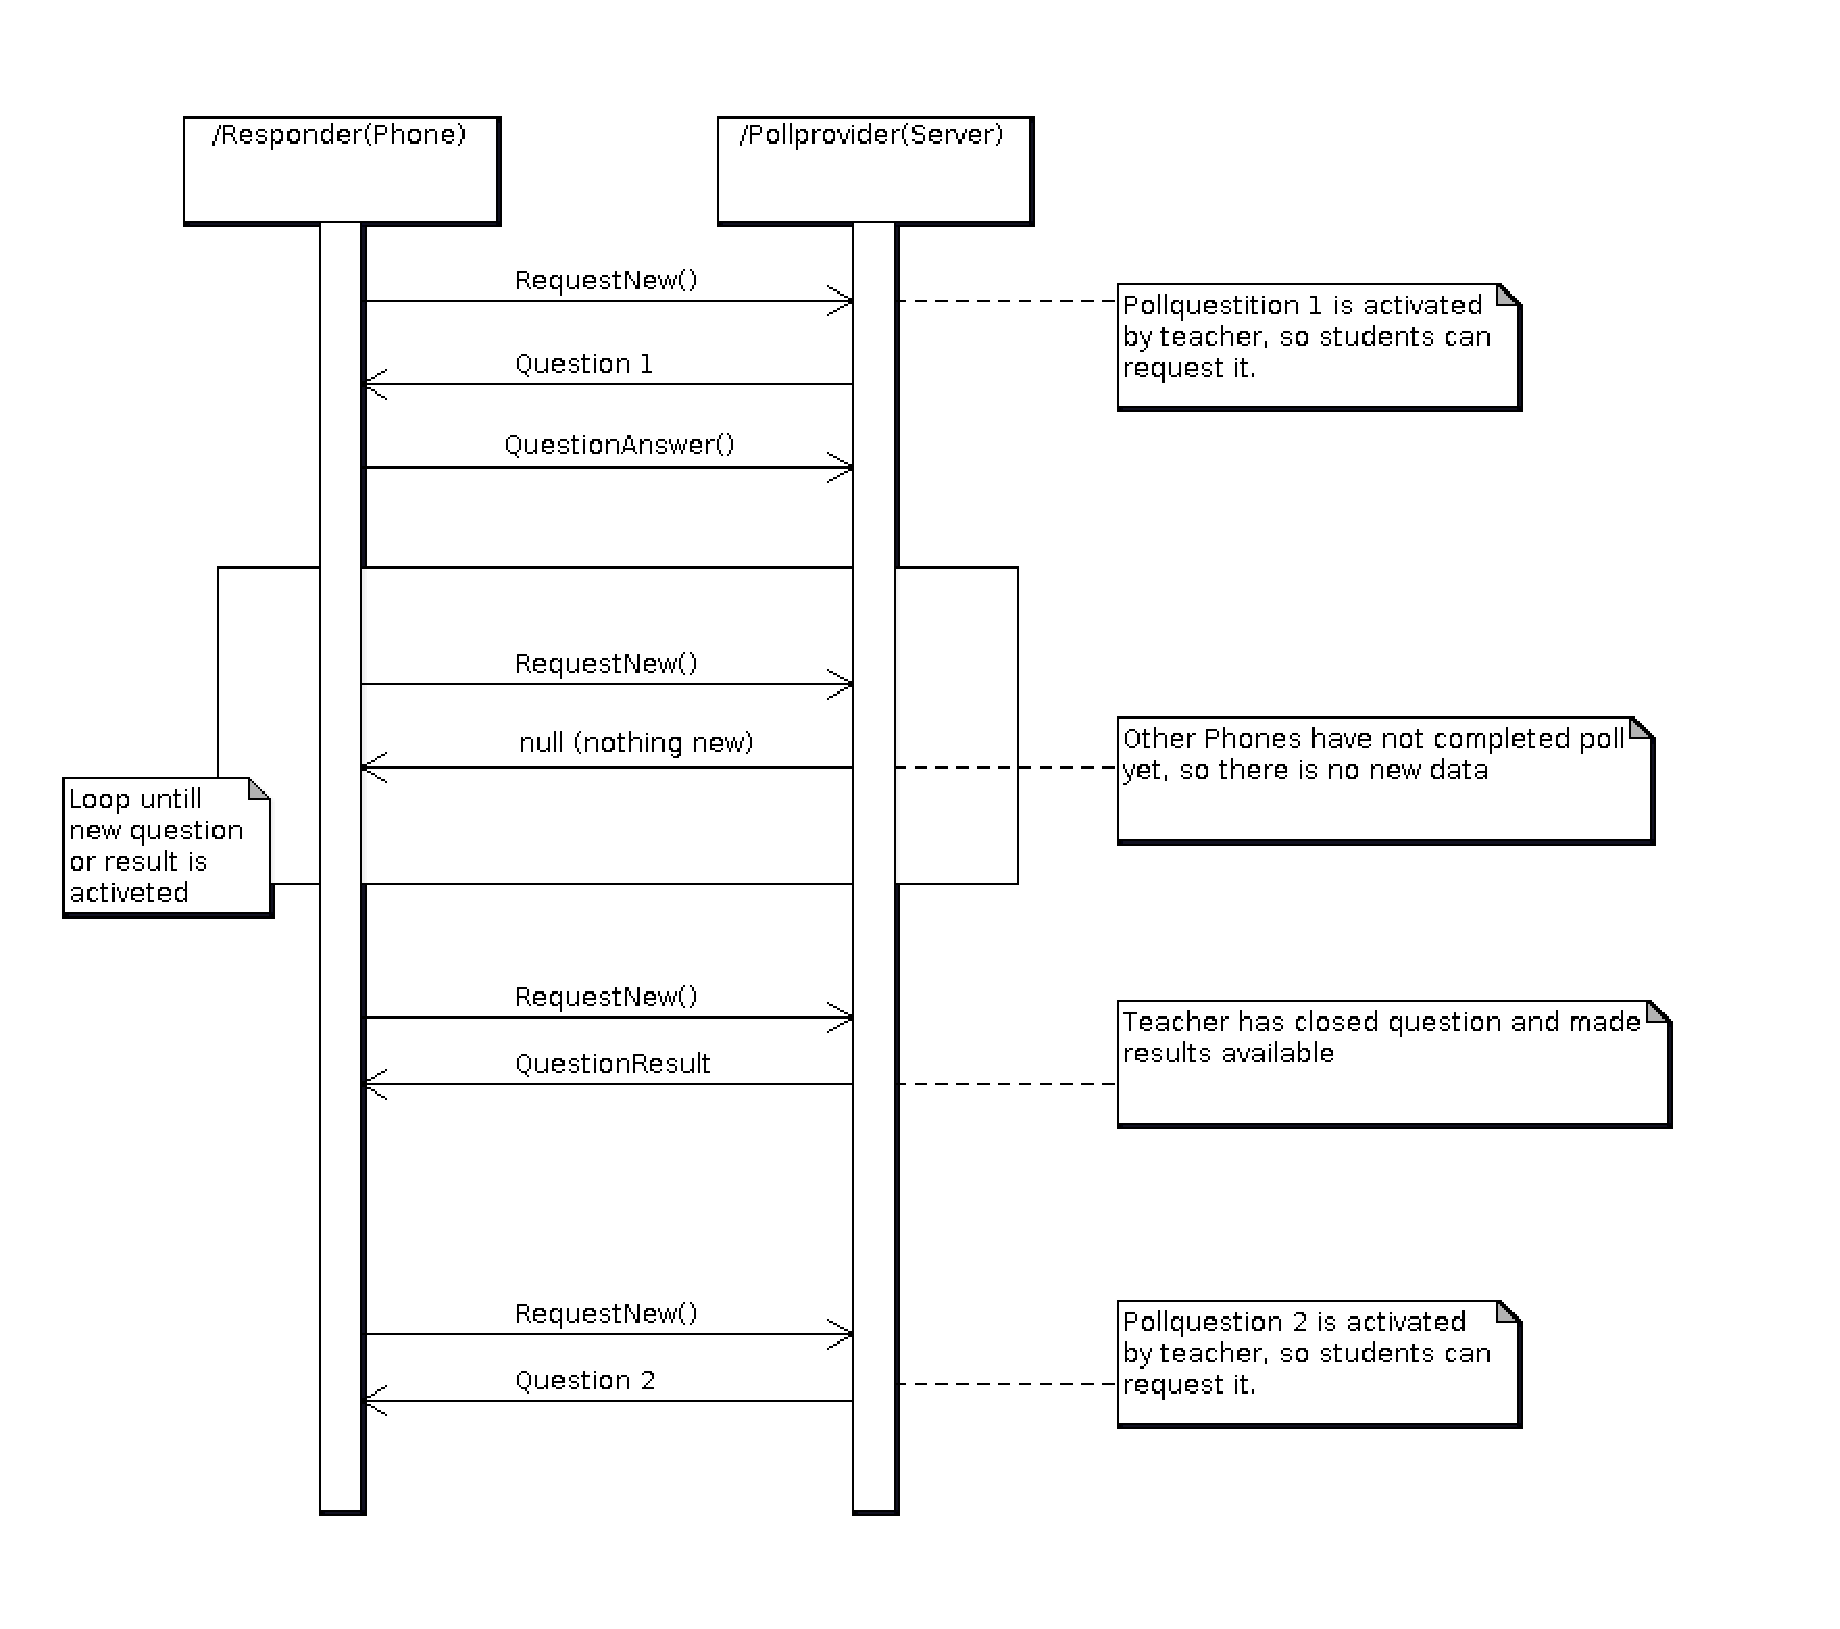
\epsfig{file=fig/Messageflow.eps, width=250px}
\caption{Message flow}
\label{fig:Messageflow}
\end{figure}


All interaction in the system is initiated by the responder
A poll consists of a several questions and possibly some answers. Each poll has an id.

In effect, the responder polls the the server to see if there is new questions/answers available.
It does this by polling the pollprovider with a \emph{RequestNew} request. If there is nothing new, it will simple get a null value back.

If there is a new question available, the responder will get a \emph{Question} back.
This package contains all the info that the responder need to present the question for the student

When the student has filled out the \emph{Question Answer}, the responder returns it to the pollprovider.
He thereafter returns to sending \emph{RequestNew} requests to the server.

At some point the question is closed by the teacher and the \emph{QuestionAnswer} is released.
When the responder polls again with \emph{RequestNew} it will get the \emph{QuestionAnswer} which is displayed to the student.

When the student has looked over the \emph{QuestionAnswer} he dismisses it and his responder returns to polling with
\emph{RequestNew} requests. At some point the next \emph{Question} is released by the teacher and the process repeats.


\begin{figure}[h]
\centering
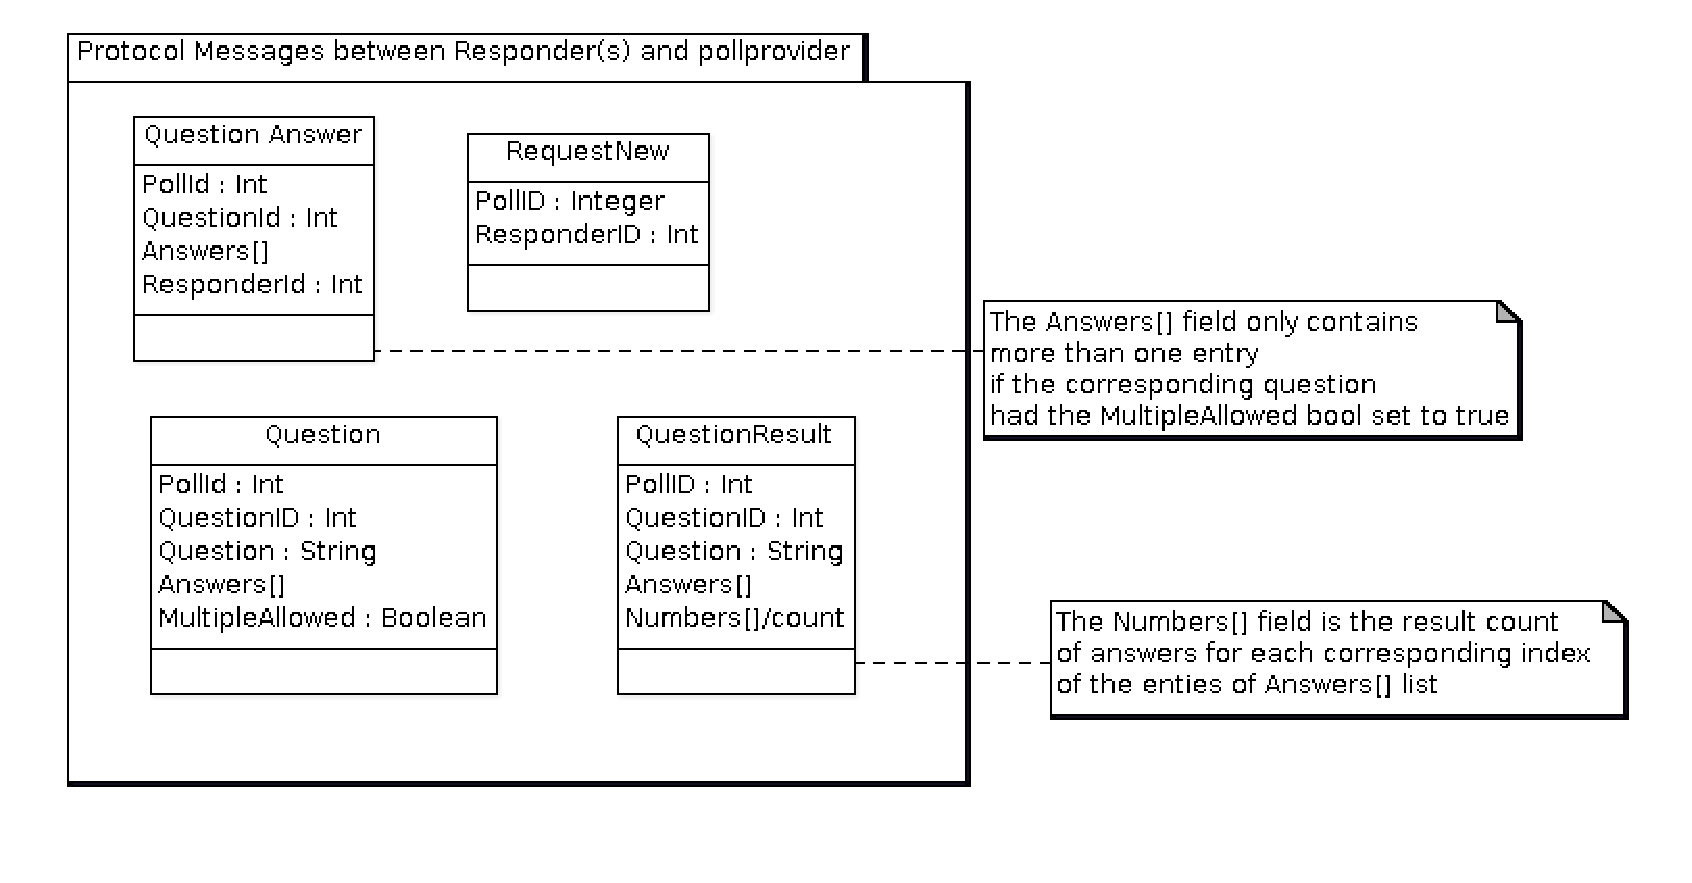
\epsfig{file=fig/ProtocolMessages.eps, width=250px}
\caption{Protocol Messages}
\label{fig:ProtocolMessages}
\end{figure}

\subsection{RequestNew}
This request is sent by the responder in hope of getting updates. It only has two attributes.
It will return a \emph{Question}, a \emph{QuestionResult} or null value if there is no new updates.

\begin{itemize}
\item PollId: The id that the teacher has assigned a specific poll. He has given this id to all students so that they may connect to the correct poll.
\item ResponderId: A unique id for the responder. The pollprovider uses this id to make sure no responder gets the same question twice.
\end{itemize}


\subsection{Question}
This package is sent as a response to a \emph{RequestNew} request. It contains a question ready for the student to answer.

\begin{itemize}
\item PollId: Id to make sure that the responder is in the right poll. Teacher might have two polls simultaneously
\item  QuestionId: a number that is incremented. Used by the responder to make sure that it the answer is sent to the right question.
\item  Quesiton: Human readable question given by the teacher.
\item  Answers[]: An array of possible answers. Forinstance [1,2,6,10] or [a,b,c,d]
\item MultipleAllowed: Attribute is set when student is allowed to check several answers (check all that applies)
\end{itemize}

\emph{QuestionAnswer}
The resquest send by the responder to the pollprovider to answer a given *Question*
\begin{itemize}
\item PollId: Identifies the poll.
\item QuestionId: Identifies the Question in the poll we are answering.
\item Answers[]: Array containing the answers. If there is only one answer, it is simply an array of one.
\item ResponderId: Id to make sure the pollprovider does not recieve answers from responders that has not retrieved the question - and to make sure no responder mistakenly answers twice.
\end{itemize}


\subsection{QuestionResult}
This package is sent as a responce to a \emph{RequestNew} request. It contains the answer to the previous \emph{Questions}

\begin{itemize}
\item PollId: The poll we are in
\item Question: The same text as in the \emph{Question} that the student answered.
\item QuestionId: Id of the \emph{Question} that this result is in relation to.
\item Answers[]: The array of answerspossibilities. that a responder could choose in the *Question*
\item Numbers[]: The array of students-that-answered-what-to-each-valid-answerpossibility
\end{itemize} 
Example: If the answerpossibilities was {a,b,c,d} and
2 students answered a, 5 answered b, 0 answered c and 1337 answered d - the Answers[] and Numbers[] attribute would have the form:
Answers{a,b,c,d}
Numbers{2,5,0,1337}
 
\section{Discussion}
\thispagestyle{fancy}% sets the current page style to 'fancy' -- must 

Security concerns/login considerations:

Student authentication is based around a unique poll ID. This ID gets generated at poll creation time. Polls can optionally be protected by a password.

The users having an android phone can access the poll (collection of questions) with the unique number supplied by the teacher. Laptop users can access the poll by putting in the same number on the webpage.

For the teacher to be able to modify the polls later in the process, an admin link is provided via email when the poll is created. This requires the teacher to supply a valid email address.

The are fuzzy thoughts about whether a device is able to vote twice, and how this is handled. A challenge response captcha is a suggestion.


\appendix

\section{Thoughs}
Test different screen sizes

\section{Revision history}
\subsection{Version 1.0}
Initial document release
\subsection{Version 1.1}
Added "MessageFlow and Protecol Messages" section

\section{Authors}
\label{app:authors}
%TODO
\begin{itemize}
\item Kim Rostgaard Christensen  s084283@student.dtu.dk
\item Jeppe Mariager s093253@student.dtu.dk
\item Jesper Kristensen s062397@student.dtu.dk
\item Hauke Petersen s101575@student.dtu.dk
\item Christian Emil Rentzmann Sonne s050436@student.dtu.dk
\item Mikko Berggren Ettienne s070168@student.dtu.dk
\item Søren Juhl Vind s062428@student.dtu.dk
\item Peter Gammelgaard Poulsen s093263@student.dtu.dk
\item Bo Visfeldt s101985@student.dtu.dk
\item Rabie Khodr Jradi s072470@student.dtu.dk
\end{itemize}


% The following two commands are all you need in the
% initial runs of your .tex file to
% produce the bibliography for the citations in your paper.
\bibliographystyle{plain}
%\nocite{*}
\bibliography{sigproc}  % sigproc.bib is the name of the Bibliography in this case
% You must have a proper ".bib" file
%  and remember to run:
% latex bibtex latex latex
% to resolve all references
%
% ACM needs 'a single self-contained file'!
%
%APPENDICES are optional


%Appendixes; Appendixes holds, for example, results or figures that are not
%relevant to place in the body of the report. Appendixes should generally be
%avoided and might not be read by the course staff.


\end{document}
